\section{Tests and Results}

\subsection{Results Exact Method}
	The result igureof Exact method in table\ref{tab:ExactMethodResults} comes from the execution of eight time the program in order to have a better estimate for the time in seconds.

	\begin{table}[h]
		\centering
		\begin{tabular}{lrrr}
			\toprule
			\textbf{Instance} & \textbf{Obj. Value} & \textbf{User Time (s)} & \textbf{Avg. CPU time (s)} \\
			\midrule
			\verb|tsp12| & 66.40 & 0.085 & 0.240 \\
			\verb|tsp60| & 629.80 & 11.240 & 36.129 \\
			\verb|rnd60| & 311.97 & 8.022 & 27.833 \\
			\verb|fb60|	& 240.47 & 24.498 & 61.198 \\
			\verb|rnd80| & 348.11 & 17.765 & 54.858 \\
			\verb|fb80| & 219.37 & 95.216 & 261.729 \\
			\verb|rnd100| & 370.09 & 30.247 & 85.942 \\
			\verb|rnd100_2| & 457.54 & 57.178 & 174.448 \\
			\verb|fb100| & 276.55 & 106.757 & 286.079 \\
			\bottomrule
		\end{tabular}
		\caption{\label{tab:ExactMethodResults} Results Exact method}
	\end{table}

	There isn't much to say about the exact method results. From the results (table~\ref{tab:ExactMethodResults}) we can see as expected that there is a trend where the increase of the number of nodes increase exponentially the CPU time (figure~\ref{fig:em-results-time}). This is not always the case, in fact the time depends a lot by the instance and the type of the instance, \verb|fb| require always more time than the other instances. The CPU time of \verb|rnd100|, \verb|rnd100_2| and \verb|fb100| show this (look at table \ref{tab:ExactMethodResults}).

	
	\begin{figure} [hb]
		\centering
		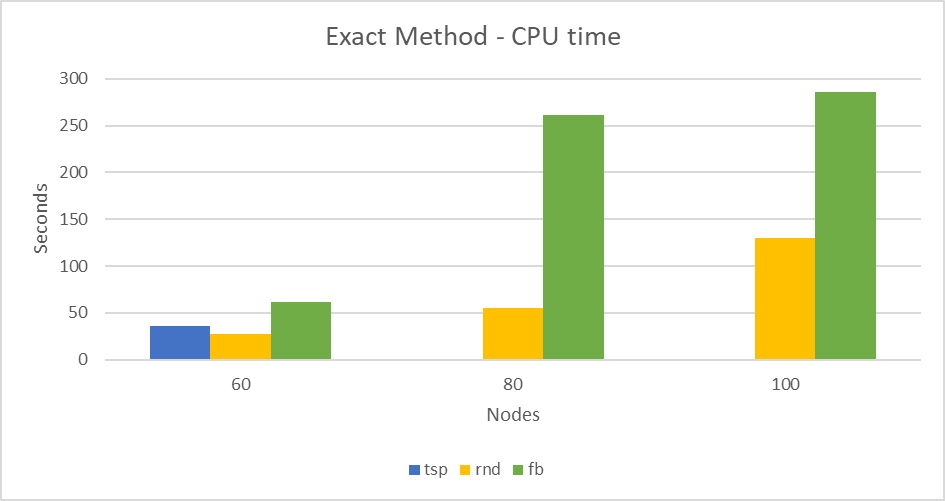
\includegraphics[width=\linewidth]{img/EM-results-time}
		\caption{Exact Method average CPU time for each instance}
		\label{fig:em-results-time}
	\end{figure}
	
	
	
\newpage
\subsection{Results Local Search}
\label{subsec:results-ls}
	The Local Search is tremendously fast but at a cost of found the optimal solution only in some instance and in average it performs poorly in comparison with other methods. In this test the User time is ignore as it is equal to CPU time, no parallel computation was implemented into meta heuristics algorithms.

	It's interesting to note the average result of Local Search. I run the LS Best Improvement (BI) and LS First Improvement (FI) with 8 random initial solution for each instance. The average results show that FI is almost always the better choice at a cost of a bit more time, that is the time needed to explore more solutions.
	
	A \textbf{good strategy} for use Local Search is to start from a lot of different initial solution, in the table~\ref{tab:LS-BestStrategyResult} I summarized the results of this strategy, every local search is started with eight different random solution and the \textbf{best value} found is selected. The \textbf{CPU time} corresponds to the sum of the time of all tabu searches ran for each instance.
	
	An interesting fact that I observed is illustrated in the figure~\ref{fig:ls-convergence}, where it's shown that with the \verb|fb| instances we have a faster convergence than in the others.
	
	\vspace{2cm}
	
	\begin{figure}[hb]
		\centering
		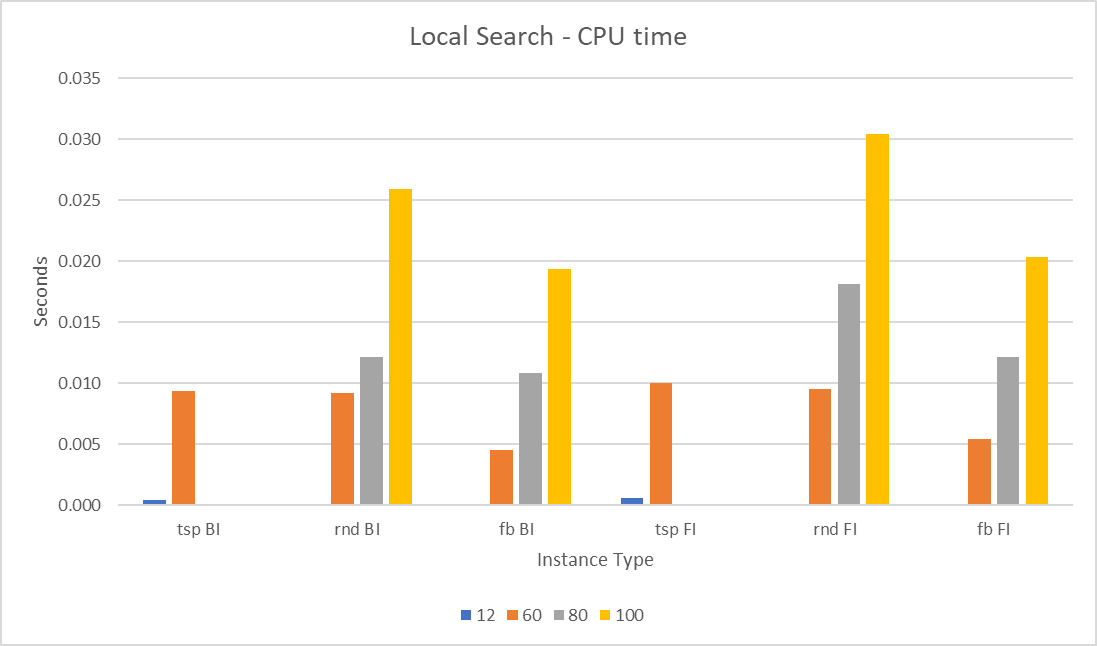
\includegraphics[width=\linewidth]{img/LS-time}
		\caption{Local Search time for each instance for each feature (BI or FI)}
		\label{fig:ls-time}
	\end{figure}

\newpage
	
	\begin{figure}[H]
		\centering
		
		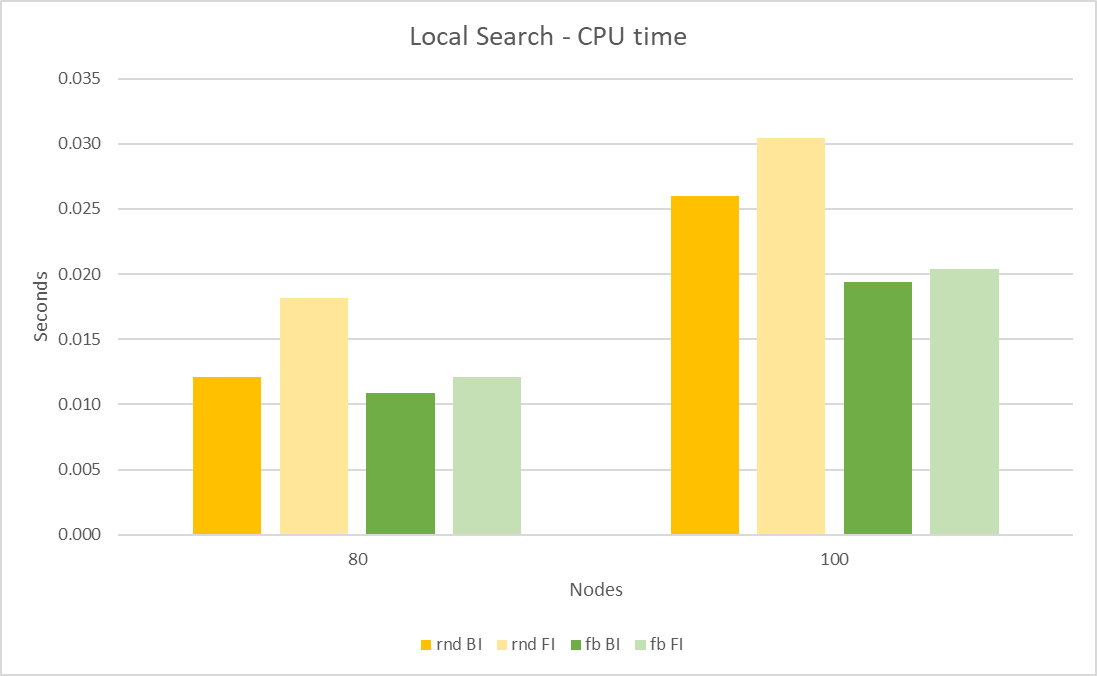
\includegraphics[width=\linewidth]{img/LS-convergence}
		
		\vspace{1cm}
		
		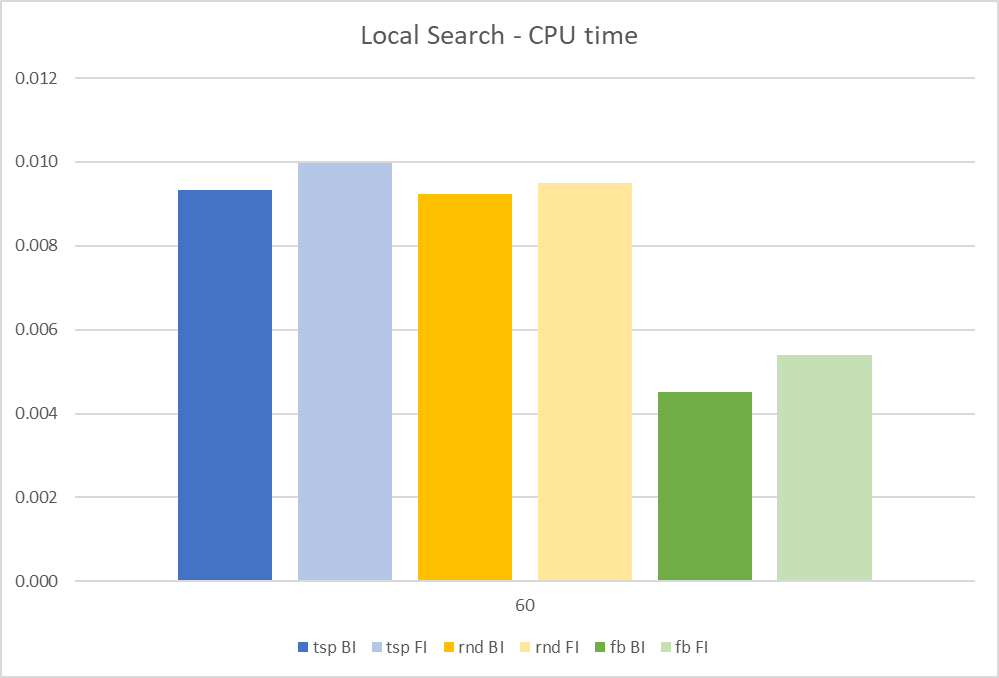
\includegraphics[width=\linewidth]{img/LS-convergence60}
		
		\caption{The faster convergence of fb instances respect to the others.}
		\label{fig:ls-convergence}
	\end{figure}
	
\newpage
	
	\begin{table}[H]
		
		\begin{tabular}{llrrr}
			\toprule
			\textbf{Instance} & \textbf{Feature} & \textbf{Avg Value} & \textbf{Avg Time (s)} & \textbf{Avg Quality} (\%) \\
			\midrule
			\verb|tsp12| 	& Best Improv. & 66.850 & 4.125e-05 & 98.3 \\
			& First Improv. & 67.325 & 7.3875e-05 & 98.6 \\
			\midrule
			\verb|tsp60| 	& Best Improv. & 666.650 & 0.00071163 & 94.5 \\
			& First Improv. & 657.362 & 0.00101625 & 95.8 \\
			\midrule
			\verb|rnd60| 	& Best Improv. & 332.826 & 0.00073738 & 93.7 \\
							& First Improv. & 329.934 & 0.00096238 & 94.6 \\
			\midrule
			\verb|fb60|		& Best Improv. & 255.999 & 0.00056363 & 93.9 \\
							& First Improv. & 256.786 & 0.00067400 & 93.6 \\ 
			\midrule
			\verb|rnd80| 	& Best Improv. & 374.400 & 0.00129013 & 93.0 \\
							& First Improv. & 371.325 & 0.00198488 & 93.7 \\
			\midrule
			\verb|fb80|		& Best Improv. & 228.525 & 0.00135700 & 95.9 \\
							& First Improv. & 233.497 & 0.00151600 &  93.9 \\
			\midrule
			\verb|rnd100| 	& Best Improv. & 406.499 & 0.00266875 & 91.0 \\
							& First Improv. & 391.406 & 0.00358875 & 94.6 \\
			\midrule
			\verb|rnd100_2| & Best Improv. & 495.690 & 0.00230150 & 92.3 \\
							& First Improv. & 492.135 & 0.00302388 & 93.0 \\
			\midrule
			\verb|fb100| & Best Improv. & 296.774 & 0.00242475 & 93.2 \\
						& First Improv. & 291.699 & 0.00254362 & 95.1 \\
			\bottomrule
		\end{tabular}
		\caption{\label{tab:AvgResultLS}Average results of all Local Search BI and FI executed}
	\end{table}
	
	\begin{table}[H]
		\centering
		\begin{tabular}{llrrr}
			\toprule
			\textbf{Instance} & \textbf{Feature} & \textbf{Best Value} & \textbf{Tot Time (s)} & \textbf{Quality (\%)} \\
			\midrule
			\verb|tsp12| & Best Improv. & 66.4 & 0.000415 & 100 \\
							& First Improv. & 66.4 & 0.000610 & 100 \\
			\midrule
			\verb|tsp60| 	& Best Improv. & 634.6 & 0.009326 & 99.2 \\
							& First Improv. & 638.6 & 0.009972 & 98.6 \\
			\midrule
			\verb|fb60|		& Best Improv. & 243.74 & 0.004509 & 98.6 \\
							& First Improv. & 243.47 & 0.005392 & 98.8 \\ 
			\midrule
			\verb|rnd60| 	& Best Improv. & 319.35 & 0.009223 & 97.7 \\
							& First Improv. & 314.53 & 0.009503 & 99.2 \\
			\midrule
			\verb|rnd80| 	& Best Improv. & 351.69 & 0.012120 & 99.0 \\
							& First Improv. & 351.05 & 0.018155 & 99.1 \\
			\midrule
			\verb|fb80| 	& Best Improv. & 223.9 & 0.010856 & 97.9 \\
							& First Improv. & 224.35 & 0.012128 & 97.7 \\
			\midrule
			\verb|rnd100| 	& Best Improv. & 387.45 & 0.028099 & 95.5 \\
							& First Improv. & 372.25 & 0.033198 & 99.4 \\
			\midrule
			\verb|rnd100_2| & Best Improv. & 476.34 & 0.023825 & 96.1 \\
							& First Improv. & 483.14 & 0.027648 & 94.7 \\
			\midrule
			\verb|fb100| & Best Improv. & 280.37 & 0.019398 & 98.6 \\
						& First Improv. & 282.99 & 0.020349 & 97.7 \\
			\bottomrule
		\end{tabular}
		\caption{\label{tab:LS-BestStrategyResult} Results of Local Search with Best Improvement and First Improvement, the result selected are only the best found from eight random initial solution}
	\end{table}
	
\newpage
\subsection{Results Tabu Search}
	
	\subsubsection{Calibration}
	\label{subsec:calibration}
	For calibration of the Tabu Search algorithm I look only to the tabu list length parameter. Hence I evaluate the test by the result obtained in \textbf{30 seconds} (CPU time),  every calibration test was be done with 30 seconds time-out. Note that if we increase the size of tabu list we need more time for check if one Move is a tabu.
	
	I tested the following instances (\verb|.dat|):
	\begin{itemize}
		\item \verb|tsp60|
		\item \verb|rnd80|
		\item \verb|fb80|
		\item \verb|rnd100|
	\end{itemize}
	
	The results of calibration phase are summarized in the charts \ref{fig:ts-calibration-rnd80} and \ref{fig:ts-calibration-rnd100}. In the Y axe we have the average of Objective value, in the X axe we have the tabu length.
	
	From these charts we can see that:
	\begin{itemize}
		\item With a large tabu length the aspiration criteria reduce the average obj. values;
		\item Different instances produce different result with the same tabu length;
		\item Long tabu length is better for instances with more nodes, this is the case for \verb|fb80| and \verb|rnd100|. For \verb|rnd80| instead we have better result only if there are aspiration criteria enabled;
		\item Long tabu length makes the average result worse in small instance: \verb|tsp60|;
		\item There are only little differences between Best Improvement and First Improvement. 
	\end{itemize}
	
	From these consideration I chose to test tabu search with three type of length:
	\begin{itemize}
		\item Small: 100;
		\item Medium: 180 (the best choice from calibration result);
		\item Large: 240;
	\end{itemize}
	Since Aspiration Criteria sometimes improve the solutions \ref{fig:ts-calibration-rnd80} and there are not marked differences between Best improvement and First Improvement I will test only tabu search with \textbf{Best Improvement} and \text{Apiration Criteria}
	
	
	\begin{figure}[p]
		\centering
		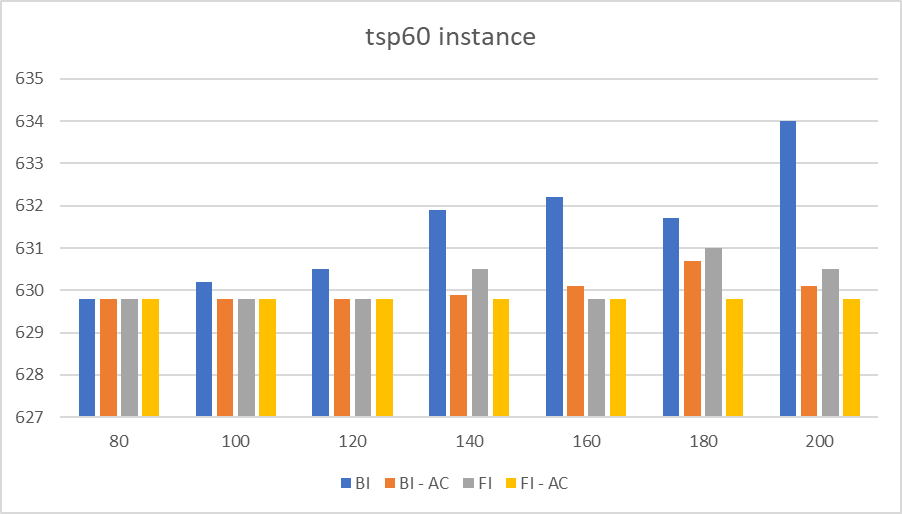
\includegraphics[width=\linewidth]{img/TS-calibration-tsp60}
		%\caption{}
		%\label{fig:ts-calibration-tsp60}
	%\end{figure}
	
	\vspace{2cm}
	
	%\begin{figure}
		%\centering
		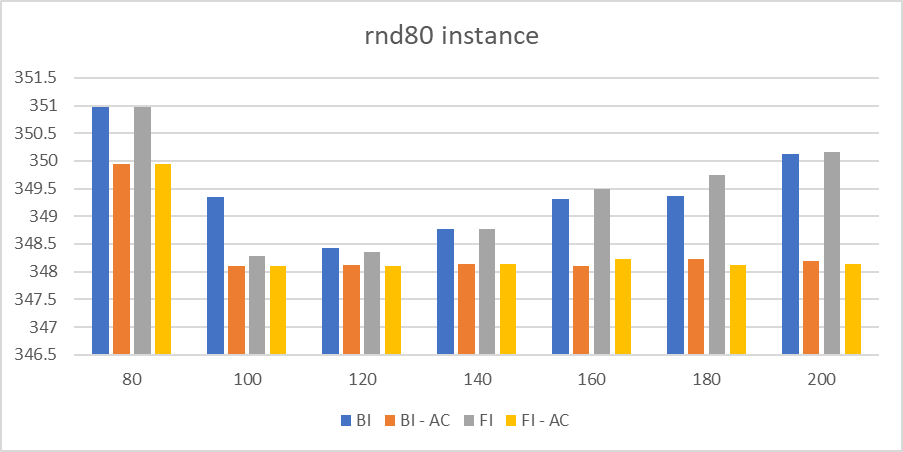
\includegraphics[width=\linewidth]{img/TS-calibration-rnd80}
		\caption{Comparison between the different Tabu length for tsp60 and rnd80 instances.}
		\label{fig:ts-calibration-rnd80}
	\end{figure}

	
	\begin{figure}[p]
		\centering
		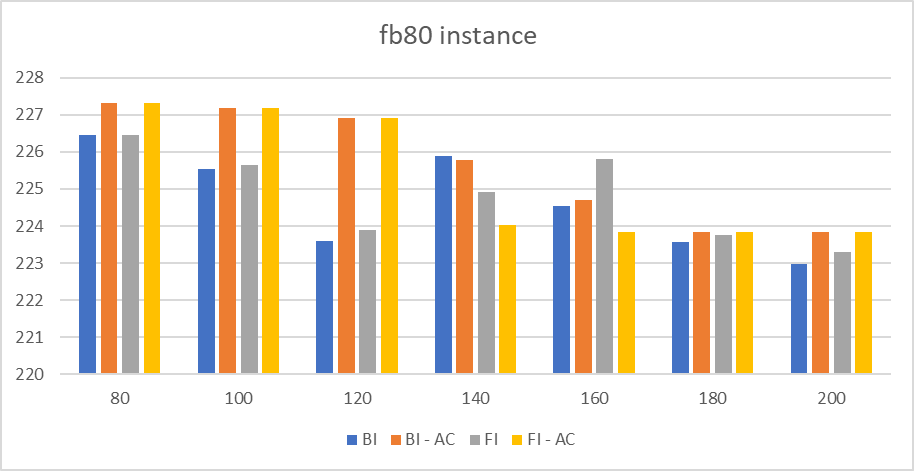
\includegraphics[width=\linewidth]{img/TS-calibration-fb80}
		%\caption{}
		%\label{fig:ts-calibration-fb80}
	%\end{figure}
	
	\vspace{2cm}
	
	%\begin{figure}
		%\centering
		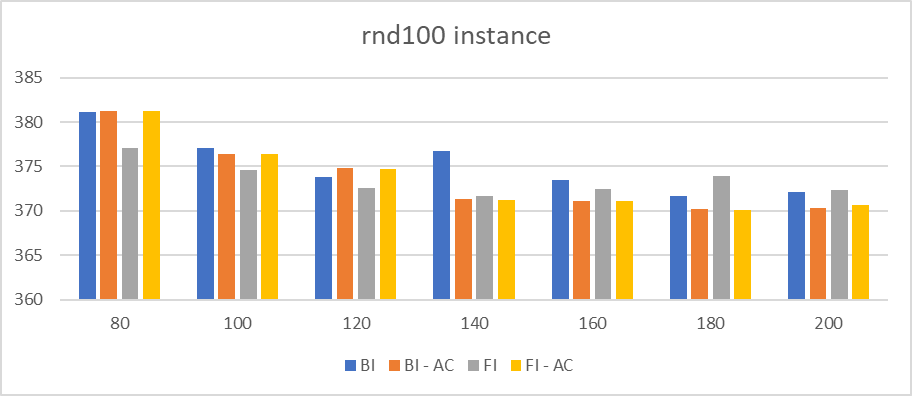
\includegraphics[width=\linewidth]{img/TS-calibration-rnd100}
		\caption{Comparison between the different Tabu length for fb80 and rnd100 instances.}
		\label{fig:ts-calibration-rnd100}
	\end{figure}
	
%	\begin{figure}[bh]
%		\centering
%		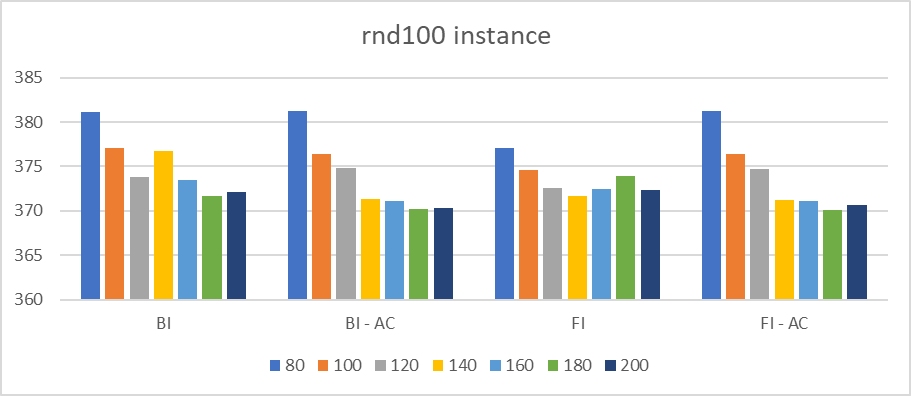
\includegraphics[width=\linewidth]{img/TS-calibration-rnd100_2}
%		\caption{Comparison between the different Tabu settings for rnd100 instance.}
%		\label{fig:ts-calibration-rnd1002}
%	\end{figure}

\newpage

	\subsubsection{Tests}
		I tested the Tabu Search implementation with three different strategy.
		
		\paragraph{Strategy 1} The Tabu Search is set as explained in the calibration phase~\ref{subsec:calibration}. The CPU time set is 30 seconds. We can see that in the case of small instance (60 nodes) the tabu with 100 of length found a better solution than the tabu with length of 180. Interesting also in the \verb|rnd100_2| instance with length of 100 we get a better solution. If we look at the optimal results \ref{tab:ExactMethodResults} we see that these better solutions are de facto the optimal solutions.
		
		\paragraph{Strategy 2} In this strategy I try to do diversification, I start 4 Tabu search with 3 different initial random solutions, the total time is 30 seconds, hence 10 seconds for each tabu search executed. From the result we can see that this strategy in some cases can improve the result found in the previously strategy. Accordingly to that is better to call multiple Tabu Search with different initial solution instead of one, in the same amount of time.
		
		\paragraph{Strategy 3} In the third strategy instead I only increase the number of CPU time from 30 to 60 second in order to see if Tabu search improve results that are not optimal. In table~\ref{tab:ts-results} we can see that this is not the case, for all the instances increasing  time of 30 seconds did not improve the best value found with \textbf{Strategy 1}.
		
		\paragraph*{} From the table \ref{tab:ts-results} we can see that the \textbf{Strategy 2} is the best, in the table \ref{tab:ts-result-q} we see that the Tabu Search found the optimum almost in all instances. From these results I think that the best ways to increase the probability to find the optimum are:
		\begin{itemize}
			\item execute more than one Tabu Search with different random initial solutions;
			\item execute Tabu Search with different tabu length.
		\end{itemize}
		
		\vspace{1cm}
		
		\begin{table}[h]
			\centering
			\begin{tabular}{l r r r}
				\toprule
				\textbf{Instance \textbackslash~Length} & \textbf{100}    & \textbf{180}    & \textbf{240}    \\
				\midrule
				\verb|tsp12|                              & 66.40   & 66.40   & 66.40   \\
				\verb|tsp60|                              & 629.80  & 631.40  & 630.80  \\
				\verb|rnd60|                              & 311.97 & 312.09 & 312.09 \\
				\verb|fb60|                               & 247.95 & 247.95 & 247.95 \\
				\verb|rnd80|                              & 348.11 & 348.23 & 348.11 \\
				\verb|fb80|                               & 222.72 & 222.70  & 222.70  \\
				\verb|rnd100|                             & 376.20  & 370.09 & 370.09 \\
				\verb|rnd100_2|                           & 457.54 & 459.30  & 460.24 \\
				\verb|fb100|                              & 288.14 & 288.14 & 279.74 \\
				\bottomrule
			\end{tabular}
			\caption{Tabu Search BI with AC results with three different type of tabu length}
			\label{tab:ts-result}
		\end{table}
	
	\begin{table}[]
		\centering
		\begin{tabular}{lrrr}
			\toprule
		\textbf{Instance} & \textbf{Strategy 1} & \textbf{Strategy 2} & \textbf{Strategy 3} \\
			\toprule
		\verb|tsp12|     & 66.40               & 66.40     & 66.40     \\
		\verb|tsp60|     & 631.40              & 630.8     & 631.40      \\
		\verb|rnd60|     & 312.09              & 312.09     & 312.09    \\
		\verb|fb60|      & 247.95              & 240.47     & 247.95    \\
		\verb|rnd80|     & 348.23              & 348.11     & 348.23    \\
		\verb|fb80|      & 222.70              & 222.70     & 222.70    \\
		\verb|rnd100|    & 370.09              & 370.09     & 370.09   \\
		\verb|rnd100_2|  & 459.30              & 459.30    & 459.30     \\
		\verb|fb100|     & 288.14              & 278.56     & 288.14    \\
			\bottomrule      
		\end{tabular}
		\caption{Results of Tabu Search BI AC with the three different strategies}
		\label{tab:ts-results}
	\end{table}

	\begin{table}[]
		\centering
		\begin{tabular}{lrr}
			\toprule
			\textbf{Instance} & \textbf{Strategy 2}& \textbf{Quality (\%)}\\
			\toprule
			\verb|tsp12|           & 66.40      & 100	  \\
			\verb|tsp60|           & 630.8     & 99.8    \\
			\verb|rnd60|           & 312.09     & 99.9    \\
			\verb|fb60|            & 240.47     & 100     \\
			\verb|rnd80|           & 348.11      & 100     \\
			\verb|fb80|            & 222.70      & 98.5    \\
			\verb|rnd100|          & 370.09      & 100     \\
			\verb|rnd100_2|        & 459.30      & 99.6    \\
			\verb|fb100|           & 278.56      & 99.2        \\
			\bottomrule      
		\end{tabular}
		\caption{Quality of the result for Tabu Search with multiple start strategy}
		\label{tab:ts-result-q}
	\end{table}
		
		